\documentclass{article}
\usepackage {anysize}\marginsize {1.25in}{1.25in}{1.0in}{1.0in}
\usepackage{setspace}
\usepackage{tikz}
\usepackage{amsmath}
\usepackage{floatrow}
\usepackage{wrapfig}
\usepackage{pgfplots}
\usepackage{hyperref}
\usepackage{amsfonts}
\usepackage[at]{easylist}
\usepackage{algorithm}
\usepackage{algpseudocode}

%----------------------------------------------------------------------
\newcommand{\e}{\mathbf{z}}
\newcommand{\emeas}{\bar{\mathbf{z}}}
\newcommand{\eest}{\hat{\mathbf{z}}}
\newcommand{\eerror}{\tilde{\mathbf{z}}}
\newcommand{\econcat}{\breve{\mathbf{z}}}
\newcommand{\ol}{\mathcal{O_L}}
\newcommand{\xhat}{\hat{\mathbf{x}}}
\newcommand{\zhat}{\hat{\mathbf{z}}}
\newcommand{\x}{\mathbf{x}}
\newcommand{\Iaz}{\underline{\mathbf{I}}_{az}}

\DeclareMathOperator*{\argmin}{arg\,min}
%----------------------------------------------------------------------


\title{Multi-Agent Mapping with Relative Navigation}
\author{James Jackson, David Wheeler}

\begin{document}
\maketitle


\begin{abstract}
  % !TEX root=main.tex

\end{abstract}

\begin{spacing}{1.5}

% !TEX root=main.tex

\section{Introduction}
% Introduce the topic of multi-agent MAV networks
As Miniature Aerial Vehicles (MAVs) are becoming increasingly stable and capable agents. They have been applied in military, private and commercial enterprises in situations such as infrastructure inspection\cite{Steich2016, Ham2016}, 3D-mapping~\cite{Remondino2011}, and disaster relief\cite{Adams2011} among others.

% Talk about cooperative SLAM
As MAVs grow increasingly capable, it has become more reasonable to consider using large number of MAVs in cooperative frameworks. Many of these applications require autonomous operation in GPS-denied or GPS-degraded environments where only relative measurements to landmarks are available to provide position feedback for control and estimation.  The problem becomes further complicated as these agents must also communicate their own observations to each other to build a combined map of the environment, solve for the relative poses of the agents to one another or both. This is known as the cooperative SLAM problem.

% Introduce filter-based navigation
While cooperative SLAM has been most extensively researched in ground robots, but there have been a number of examples of cooperative SLAM on MAVs in recent literature~\cite{Loianno2015, Achtelik2012, Lawson2015}. In addition, there have been works which are marked by efforts to reduce computational requirements to perform SLAM on computationally-constrained MAV platforms with strict size, weight, and power (SWaP) requirements.  One common approach is to simplify the problem using an extended Kalman filter (EKF) to fuse interoceptive and exteroceptive sensor measurements
~\cite{Bachrach2010a, Wheeler2017b, Achtelik2009, Ahrens2009, Chowdary2013} to provide estimates of global states.

% Introduce Pose Graph optimization
One disadvantage of a global filter-based approach without global measurements is the unobservability of global position and heading states~\cite{Martinelli2012,Weiss2012,Jones2007} This causes two primary problems: global drift and inconsistency in state estimates and sub-optimal sensor fusion~\cite{Bailey2006Consistency,Bar-Shalom2002}. To correct drift, a common approach is to frame the the global trajectory as a pose graph and incorporate loop closure constraints.  The global state is then found by optimizing over poses to remove accumulated drift.  However, filter inconsistency has continued to be a documented problem in global filter-based approaches~\cite{Wheeler2017a}.

% Introduce relative navigation framework
Wheeler et al.~\cite{Wheeler2017a} shows that framing the navigation problem into a relative context can side-step state unobservability by directly measuring and controlling states with respect to observable landmarks.  Global states are then solely estimated with higher-order methods such as pose-graph optimization and are not in real-time feedback control loops.  This method has been shown to improve estimator performance both in simulation and in hardware experiments~\cite{Wheeler2017a, Wheeler2017b}.

% Connect relative Navigation and pose graph optimization
In the relative state estimation framework~\cite{Koch2017}, states are estimated with respect to a locally-observable ``keyframe'' image or laser scan.  As this keyframe goes out of view, another is declared and global position and heading states are reset to zero.  Uncertainty of these states is also reset to zero, as they are defined with respect to that keyframe, which is known with absolute certainty at the time of the reset.  The reset step in the relative estimator provides a clear mechanism to create mutually independent edge constraints for a pose graph.  Prior to the incorporation of loop closures, the vehicle's global pose can be calculated by traversing from the origin of the graph to the current keyframe, compounding edge constraints and finally adding the relative state.  Uncertainty in these states can be calculated using higher order methods such as those described by Barfoot et al. in ~\cite{Barfoot2014}.  After loop closures, global states can be calculated using pose-graph optimization techniques such as g$^2$o~\cite{Kummerle2011}, or iSAM2~\cite{Kaess2012}

% Illustrate the idea of multi-agent relative navigation
In this work, we show the multi-agent extension to relative navigation.  Because all agents using a relative estimator navigate with respect to locally-observable landmarks, real-time control is insulated from global state updates.  This means that global states can be initialized arbitrarily and experience large updates without negative consequences on real-time performance. Additionally, as the entire map is defined in terms of mutually independent relative constraints, fusing multiple maps becomes relatively trivial.  In this work, we will show the scalability of an entirely relative multi-agent system by fusing maps from over 100 agents in real time on a laptop computer.

% Introduce edge-based optimization
One drawback of global pose optimization is a strong dependence on the quality of the initialization point for the graph.  Even a small heading error in a trajectory can result in large pose errors after a long period of time.  This problem is an active area of research and there are several prominent solutions which have been proposed~\cite{Carlone2015, Kim2010a, Agarwal2014, Wang2014}.  In this work, we present a new initialization technique in which we optimize over the edge constraints in a pose graph, rather than poses in a stochastic fashion. This method is similar to SGD-MM~\cite{Wang2014}, except we use the relative states directly, as opposed to the incremental state representation.

% Overview of paper
In this paper, we will first derive relative edge optimization and formulate the relative edge optimization problem.  We will then discuss several implementation details to ensure the scalability of edge optimization.  Then, we will show results of edge optimization in a large simulation framework of 100 agents, and discuss the strengths and weaknesses of edge optimization when compared with global pose optimization.  Finally, we will show results of a hardware demonstration of four multirotor agents.

% !TEX root=main.tex

\section{Edge Optimization}

\subsection{Nomenclature}

\begin{align*}
\emeas_{ij}   & \text{: edge measurement between vertex $i$ and $j$}\\
\eest_{ij}    & \text{: current edge estimate} \\
\Delta\e_{ij} & \text{: current edge update}\\
\eest_{ij}^+  & \text{: new edge estimate}\\
\emeas_{az}   & \text{: non-sequential edge measurement (loop closure)}\\
\eest_{a-z}   & \text{: estimated edge between non-sequential vertex $a$ and $z$} \\
\eest_{a-z}^+ & \text{: new estimated edge between non-sequential vertex $a$ and $z$} \\
%
%
n & \text{: Dimension of $\e$ } \\
e & \text{: Number of odometry edges } \\
%
%
\emeas   & \text{: all edge measurements, $\in \mathbb{R}^{en}$}\\
\eest    & \text{: all edge estimates, $\in \mathbb{R}^{en}$}\\
\Delta\e & \text{: all edge updates,  $\in \mathbb{R}^{en}$}\\
%
%
\Omega_{ij} & \text{: Information matrix associated with odometry edge (inverse covariance) } \\
\Omega_{az} & \text{: Information matrix associated with loop closure edge } \\
%
%
\mathbf{x}_i & \text{: Pose of vertex $i$ with respect to global coordinate frame} \\
\mathcal{O} & \text{: Set of odometry edges} \\
\mathcal{L} & \text{: Some subset of loop closure constraints} \\
\mathcal{O_L} & \text{: Set of odometry edges that form the redundant paths of $\mathcal{L}$} \\
\end{align*}

\subsection{Global Pose Optimization}


% describe mathematically pose optimization
Pose graph optimization typically formulated as a least-squares optimization problem.  This formulation can be derived analytically from the structure of the pose graph~\cite{Kummerle2011} or from a Bayesian perspective in a factor graph~\cite{Kaess2008}.  Both derivations ultimately pose the optimization problem similar to the following:

\begin{align}
  F(\eest,\emeas) = \sum_{\{i,j\} \in \mathcal{O}} \overbrace{(\eest_{ij}-\emeas_{ij})^\top\Omega_{ij}(\eest_{ij}-\emeas_{ij})}^\text{Odometry error penalty} + \sum_{\{a,z\} \in \mathcal{L}} \overbrace{ (\eest_{a-z}-\emeas_{az})^\top \Omega_{az} (\eest_{a-z}-\emeas_{az}) }^\text{Loop error penalty}
  \label{eqn:cost_function}
\end{align}

The process then assumes the following steps:

\begin{enumerate}
  \item define an initial global pose estimate for each vertex $\xhat_i$
  \item determine the estimated edges by differencing two connected vertices $\eest_{ij} = \xhat_j - \xhat_i$
  \item find the optimal set of vertex positions to minimize the cost

  \begin{align}
      \xhat^* = \argmin_{\xhat} F\Big(\eest(\xhat),\emeas \Big)
	     \label{eqn:global_opt}
	\end{align}

  The typical approach is
		\begin{enumerate}
		\item Express the cost function in terms of $\xhat^+ = \xhat + \Delta\x$
		\item Linearize $\eest(\xhat)$ in terms of $\Delta\x$
		\item Take the partial derivative of the cost function with respect to $\Delta\x$
		\item Restructure the problem to be of the form $A \Delta \x = b$ and solve for $\Delta\x$.
		\item Apply the update to $\xhat$ and repeat steps (a)-(e) until $\Delta\x < \epsilon$.
	\end{enumerate}

\end{enumerate}

Global pose optimization solves the system by projecting onto the Cartesian coordinate frame with respect to a single pose. When only relative information is available, the initial global pose estimates can be arbitrarily far from their true position. The iterative nature of the Newton method works ideally when close to the solution, but can converge on a local minimum otherwise.


% describe mathematically edge optimization
\subsection{Relative Edge Optimization}
Instead of optimizing over poses, we propose to optimize directly over relative edge constraints $\eest$.  This avoids the use of a privileged coordinate frame like the starting point of the vehicle or the global origin and keeps the problem in the measurement space.  The optimization problem is posed as

\begin{align}
  \mathbf{\eest}^* = \argmin_{\eest} F\Big(\eest,\emeas \Big).
  \label{eqn:relative_opt}
\end{align}

In contrast to Equation \ref*{eqn:global_opt}, it becomes clear that global vertex positions are never introduced. Rather, we update the original edge estimates directly. Assuming our incoming odometry measurements are zero-mean, setting $\eest_0 = \emeas$ will be a good initial guess.

We wish to find the optimal update $\Delta\e^*$ to our initial edge estimate. Letting $\eest^+ = \eest + \Delta\e$ and $\eest_{a-z}^+ = h(\eest_{a-z},\Delta\e)$ we see
\begin{align*}
  F(\eest^+,\emeas) &= \sum_{\{i,j\} \in \mathcal{O}} (\eest_{ij} + \Delta\e_{ij}-\emeas_{ij})^\top\Omega_{ij}(\eest_{ij} + \Delta\e_{ij}-\emeas_{ij}) + \sum_{\{a,z\} \in \mathcal{L}} (\eest_{a-z}^+-\emeas_{az})^\top\Omega_{az}(\eest_{a-z}^+-\emeas_{az}) \\
  &= (\eest+\Delta\e-\emeas)^\top\boldsymbol{\Omega}(\eest+\Delta\e-\emeas) + \sum_{\{a,z\} \in \mathcal{L}} (h(\eest_{a-z},\Delta\e)-\emeas_{az})^\top\Omega_{az}(h(\eest_{a-z},\Delta\e)-\emeas_{az})
\end{align*}

where

\begin{align*}
  \boldsymbol{\Omega} &= \left[\begin{array}{ccc}
  \Omega_{01} & \mathbf{0} & \mathbf{0} \\
  \mathbf{0}  & \ddots     & \mathbf{0} \\
  \mathbf{0}  & \mathbf{0} & \Omega_{e-1,e}\\
  \end{array}\right].
\end{align*}

Taking the derivative of the cost function with respect to $\Delta\e$ and setting it equal to zero will allow us to solve for the optimal edge update $\Delta\e^*$.

Using the matrix calculus chain rule and simplifying, we see
\begin{align*}
  \dfrac{\partial F(\eest^+,\emeas)}{\partial \Delta\e} = \mathbf{0}^\top \\
  2 (\eest+\Delta\e^*-\emeas)^\top \boldsymbol{\Omega} \frac{\partial (\eest+\Delta\e-\emeas)}{\partial \Delta\e}
    + \sum_{\{a,z\} \in \mathcal{L}} 2
  (h(\eest_{a-z},\Delta\e^*)-\emeas_{az})^\top \Omega_{az}
  \frac{\partial h(\eest_{a-z},\Delta\e)}{\partial \Delta\e}
  = \mathbf{0}^\top
  \\
  (\eest+\Delta\e^*-\emeas)^\top \boldsymbol{\Omega}
  + \sum_{\{a,z\} \in \mathcal{L}}
  (h(\eest_{a-z},\Delta\e^*)-\emeas_{az})^\top \Omega_{az}
  \frac{\partial h(\eest_{a-z},\Delta\e)}{\partial \Delta\e}
  = \mathbf{0}^\top.
\end{align*}

Transpose both sides, noting that the information matrices are symmetric
\begin{align*}
  \boldsymbol{\Omega} (\eest+\Delta\e^*-\emeas)
  + \sum_{\{a,z\} \in \mathcal{L}}
  \frac{\partial h(\eest_{a-z},\Delta\e)}{\partial \Delta\e}^\top \Omega_{az} (h(\eest_{a-z},\Delta\e^*)-\emeas_{az})
  = \mathbf{0}.
\end{align*}

The first term causes the optimization to respect the odometry constraints; it is always linear with respect to $\Delta\e$ even when the underlying edges are nonlinearly coupled. The second term is a function of the set of edges found in the various loop closures $\mathcal{O_L}$. As a result, any edge not found in a loop closure can be trivially solved for directly using the first term. We see
\begin{align*}
  \Delta\e_{ij}^* = \emeas_{ij} -\eest_{ij}
  \end{align*}
  such that
  \begin{align*}
  \eest_{ij}^+ = \emeas_{ij}  \text{ for } \{i,j\} \notin \mathcal{O_L}.
\end{align*}
In other words, any edge estimate that is not part of a redundant path is driven to its original measured state. These edges do not influence the optimization, in no way pinning them to some initial Cartesian pose.   We can finally move all constant terms to the right-hand side of the equation and write the final cost function.
\begin{align}
  \boldsymbol{\Omega} \Delta\e^*  + \sum_{\{a,z\} \in \mathcal{L}}
  \frac{\partial h(\eest_{a-z},\Delta\e)}{\partial \Delta\e}^\top
  \Omega_{az}(h(\eest_{a-z},\Delta\e^*)-\emeas_{az})
  &= -\boldsymbol{\Omega}(\eest -\emeas)
  \label{eqn:opt}
\end{align}

To solve Eq.~\ref{eqn:opt}, we will linearize the system about current estimate for all edge constraints and perform Gauss-Newton optimization.  Let us define

\begin{align*}
  \mathbf{H}_{az} = \frac{\partial h(\eest_{a-z},\Delta\e)}{\partial \Delta\e} \mid_{\Delta\e = \mathbf{0}}
\end{align*}

such that the second-order approximation of the compounding of a series of edges in a non-trivial space, like $SE(2)$, can be shown as follows:

\begin{align*}
  h(\eest_{a-z},\Delta\e) &= (\eest_{ab} + \Delta\e_{ab}) \circ (\eest_{bc} + \Delta\e_{bc}) \circ ... \circ (\eest_{yz} + \Delta\e_{yz})\\
   &\approx
  h(\eest_{a-z},\mathbf{0}) + \mathbf{H}_{az} \Delta\e,
\end{align*}

and we will use the first order approximation for the partial
\begin{align*}
  \frac{\partial h(\e_{a-z},\Delta\e)}{\partial \Delta\e} &\approx \mathbf{H}_{az}.
\end{align*}

With this approximation, Equation \ref{eqn:opt} simplifies to

\begin{align}
  \left(\boldsymbol{\Omega} + \sum_{\{a,z\} \in \mathcal{L}}
  \mathbf{H}_{az}^\top
  \Omega_{az}\mathbf{H}_{az} \right) \Delta\e^*
  &= -\boldsymbol{\Omega}(\eest -\emeas) - \sum_{\{a,z\} \in \mathcal{L}}
  \mathbf{H}_{az}^\top
  \Omega_{az}(h(\eest_{a-z},\mathbf{0}) -\emeas_{az})
  \label{eqn:3d_opt}
\end{align}

\subsection{Relative Edge Optimization in $SE(2)$}

Take the example of a 3 DoF robot which follows the standard unicycle model, where edges are defined as $\e_i = \left[\begin{array}{ccc} f_i & r_i & \theta_i \end{array}\right]^\top$ where $f$ and $r$ represent forward and right motion and $\theta$ represents a change in bearing. In this case translational motion is coupled with heading. A series of edges can be represented as a series of transformation matrices as follows:

\begin{align*}
	h(\eest_{a-z},\Delta\e) =  \left[\begin{array}{c}
	T_{az,13} \\ T_{az,23} \\ \sum_{i \in \{a,z\}} \left( \theta_i + \Delta\theta_i \right)
	\end{array}\right]
\end{align*}

where

\begin{align*}
  T_{az} &= T_{ab} T_{bc} T_{cd} ... T_{yz}
\end{align*}

and

\begin{align*}
  T_{ij} &= \left[\begin{array}{ccc}
  \cos(\theta_i + \Delta\theta_i) & -\sin(\theta_i + \Delta\theta_i) & f_i + \Delta f_i \\
  \sin(\theta_i + \Delta\theta_i) &  \cos(\theta_i + \Delta\theta_i) & r_i + \Delta r_i \\ 0 & 0 & 1
  \end{array}\right]
\end{align*}

Note that bearing angle just sums between edge compounding through multiplication of the rotation part of the transform.

Let $w$ be the number of edges in the loop closure from $a-z$.
The partial derivative of compounding a series of edges is

\begin{align*}
   \mathbf{H}_{az} &=
  \left[\begin{array}{ccccccccc}
  R_{\boldsymbol{\theta}_1} & \mathbf{g}_2 & R_{\boldsymbol{\theta}_2} & \mathbf{g}_3 &
  \dots & R_{\boldsymbol{\theta}_{w-1}} & \mathbf{g}_w & R_{\boldsymbol{\theta}_w} & \mathbf{0}\\
  \mathbf{0}^\top & 1 & \mathbf{0}^\top & 1 & \dots
   & \mathbf{0}^\top & 1 & \mathbf{0}^\top & 1 \end{array}\right]
\end{align*}

where
\begin{align*}
  \boldsymbol{\theta} = \left[\begin{array}{ccc}
  \boldsymbol{\theta}_1&
  \dots&
  \boldsymbol{\theta}_{w+1}
  \end{array}\right]^\top =  \left[\begin{array}{ccccc}
  0 & \theta_{ab} & \theta_{ab} + \theta_{bc} & \dots & \sum_{i \in \{a,z\}} \left( \theta_i + \Delta\theta_i \right)
  \end{array}\right]^\top
\end{align*}

is the cumulative bearing angle,

\begin{align*}
  R_a = \left[\begin{array}{cc}
  \cos(a) & -\sin(a) \\ \sin(a) & \cos(a)
  \end{array}\right]
\end{align*}

is a rotation matrix, and

\begin{align*}
  \mathbf{g}_k = \sum_{i=k}^{w} \left(\left[\begin{array}{cc}
  -\sin(\boldsymbol{\theta}_i) & -\cos(\boldsymbol{\theta}_i) \\ \cos(\boldsymbol{\theta}_i) & -\sin(\boldsymbol{\theta}_i)
  \end{array}\right]
  \left[\begin{array}{c}
  f_i \\ r_i
  \end{array}\right]\right).
\end{align*}.

% show that they are mathematically equivalent
% describe differences (pros/cons)
% how to use them together

% !TEX root=main.tex

\section{Comparison: Relative Edge vs. Pose Optimization}

\begin{figure}
  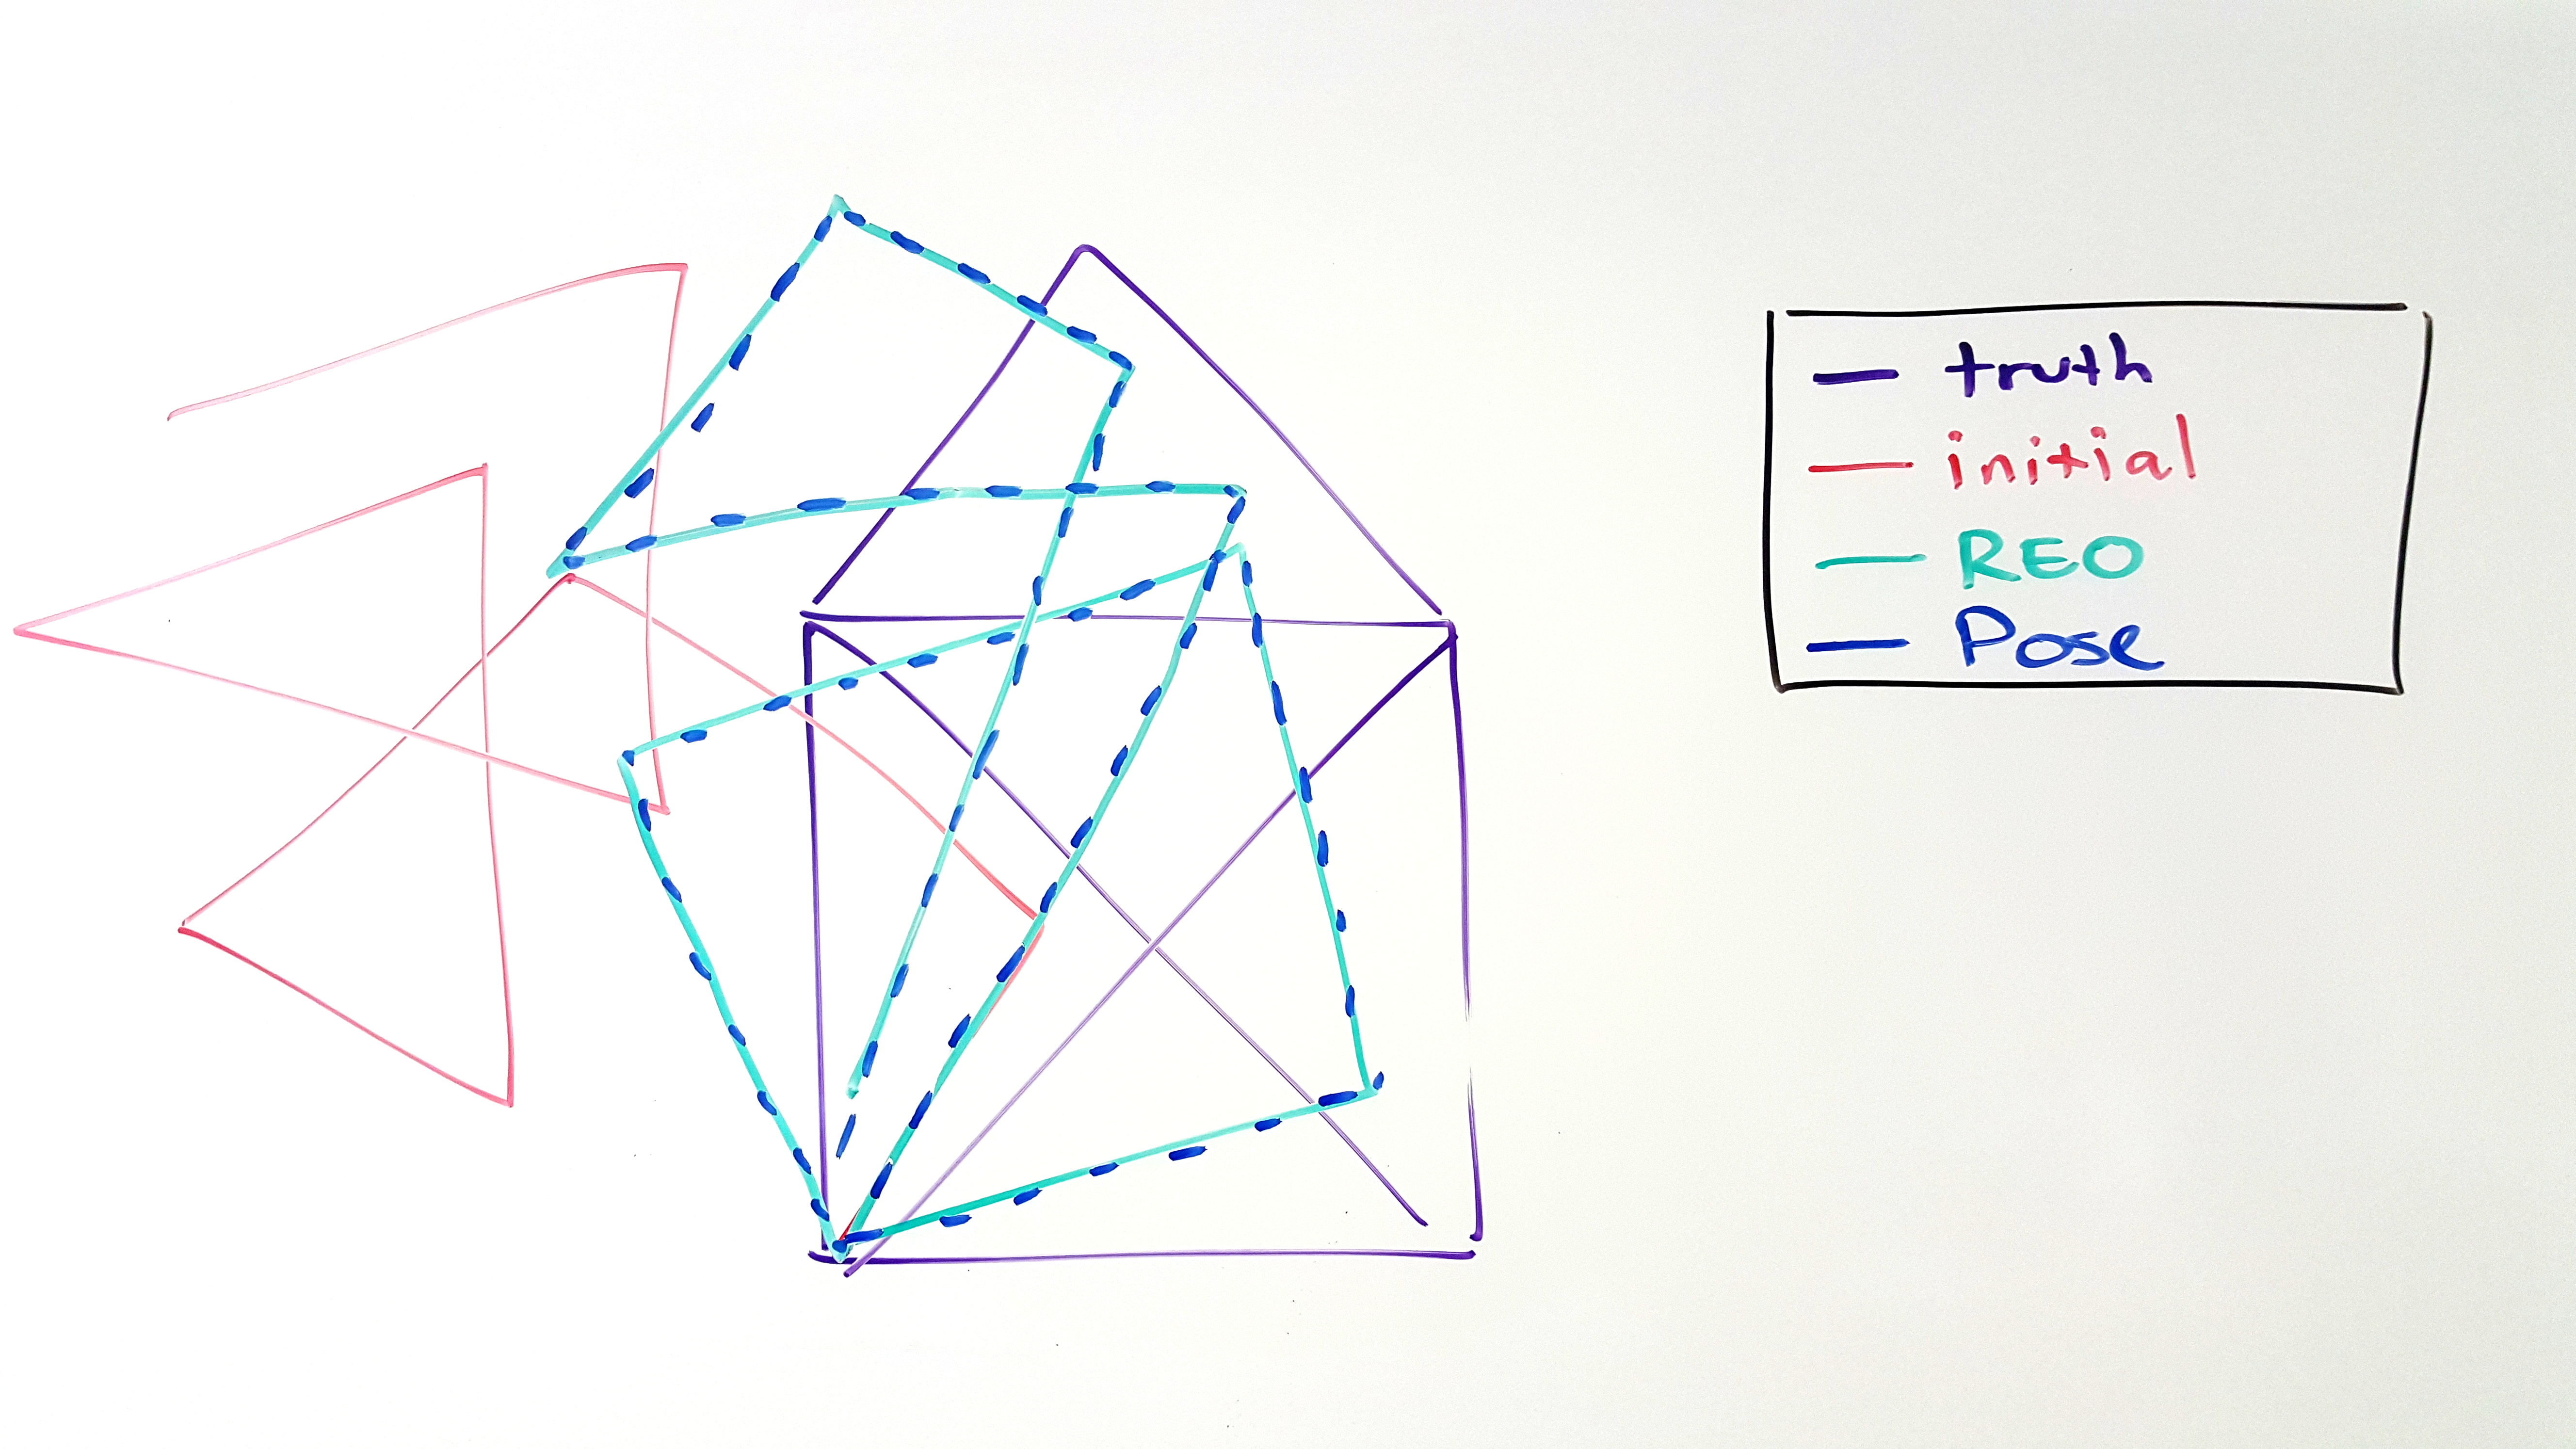
\includegraphics[width=0.7\textwidth]{figures/house_trajectory.jpg}
  \caption{One sample from a house trajectory with optimization results from relative edge optimization and global pose optimization}
  \label{fig:house_trajectory}
\end{figure}

\begin{figure}
  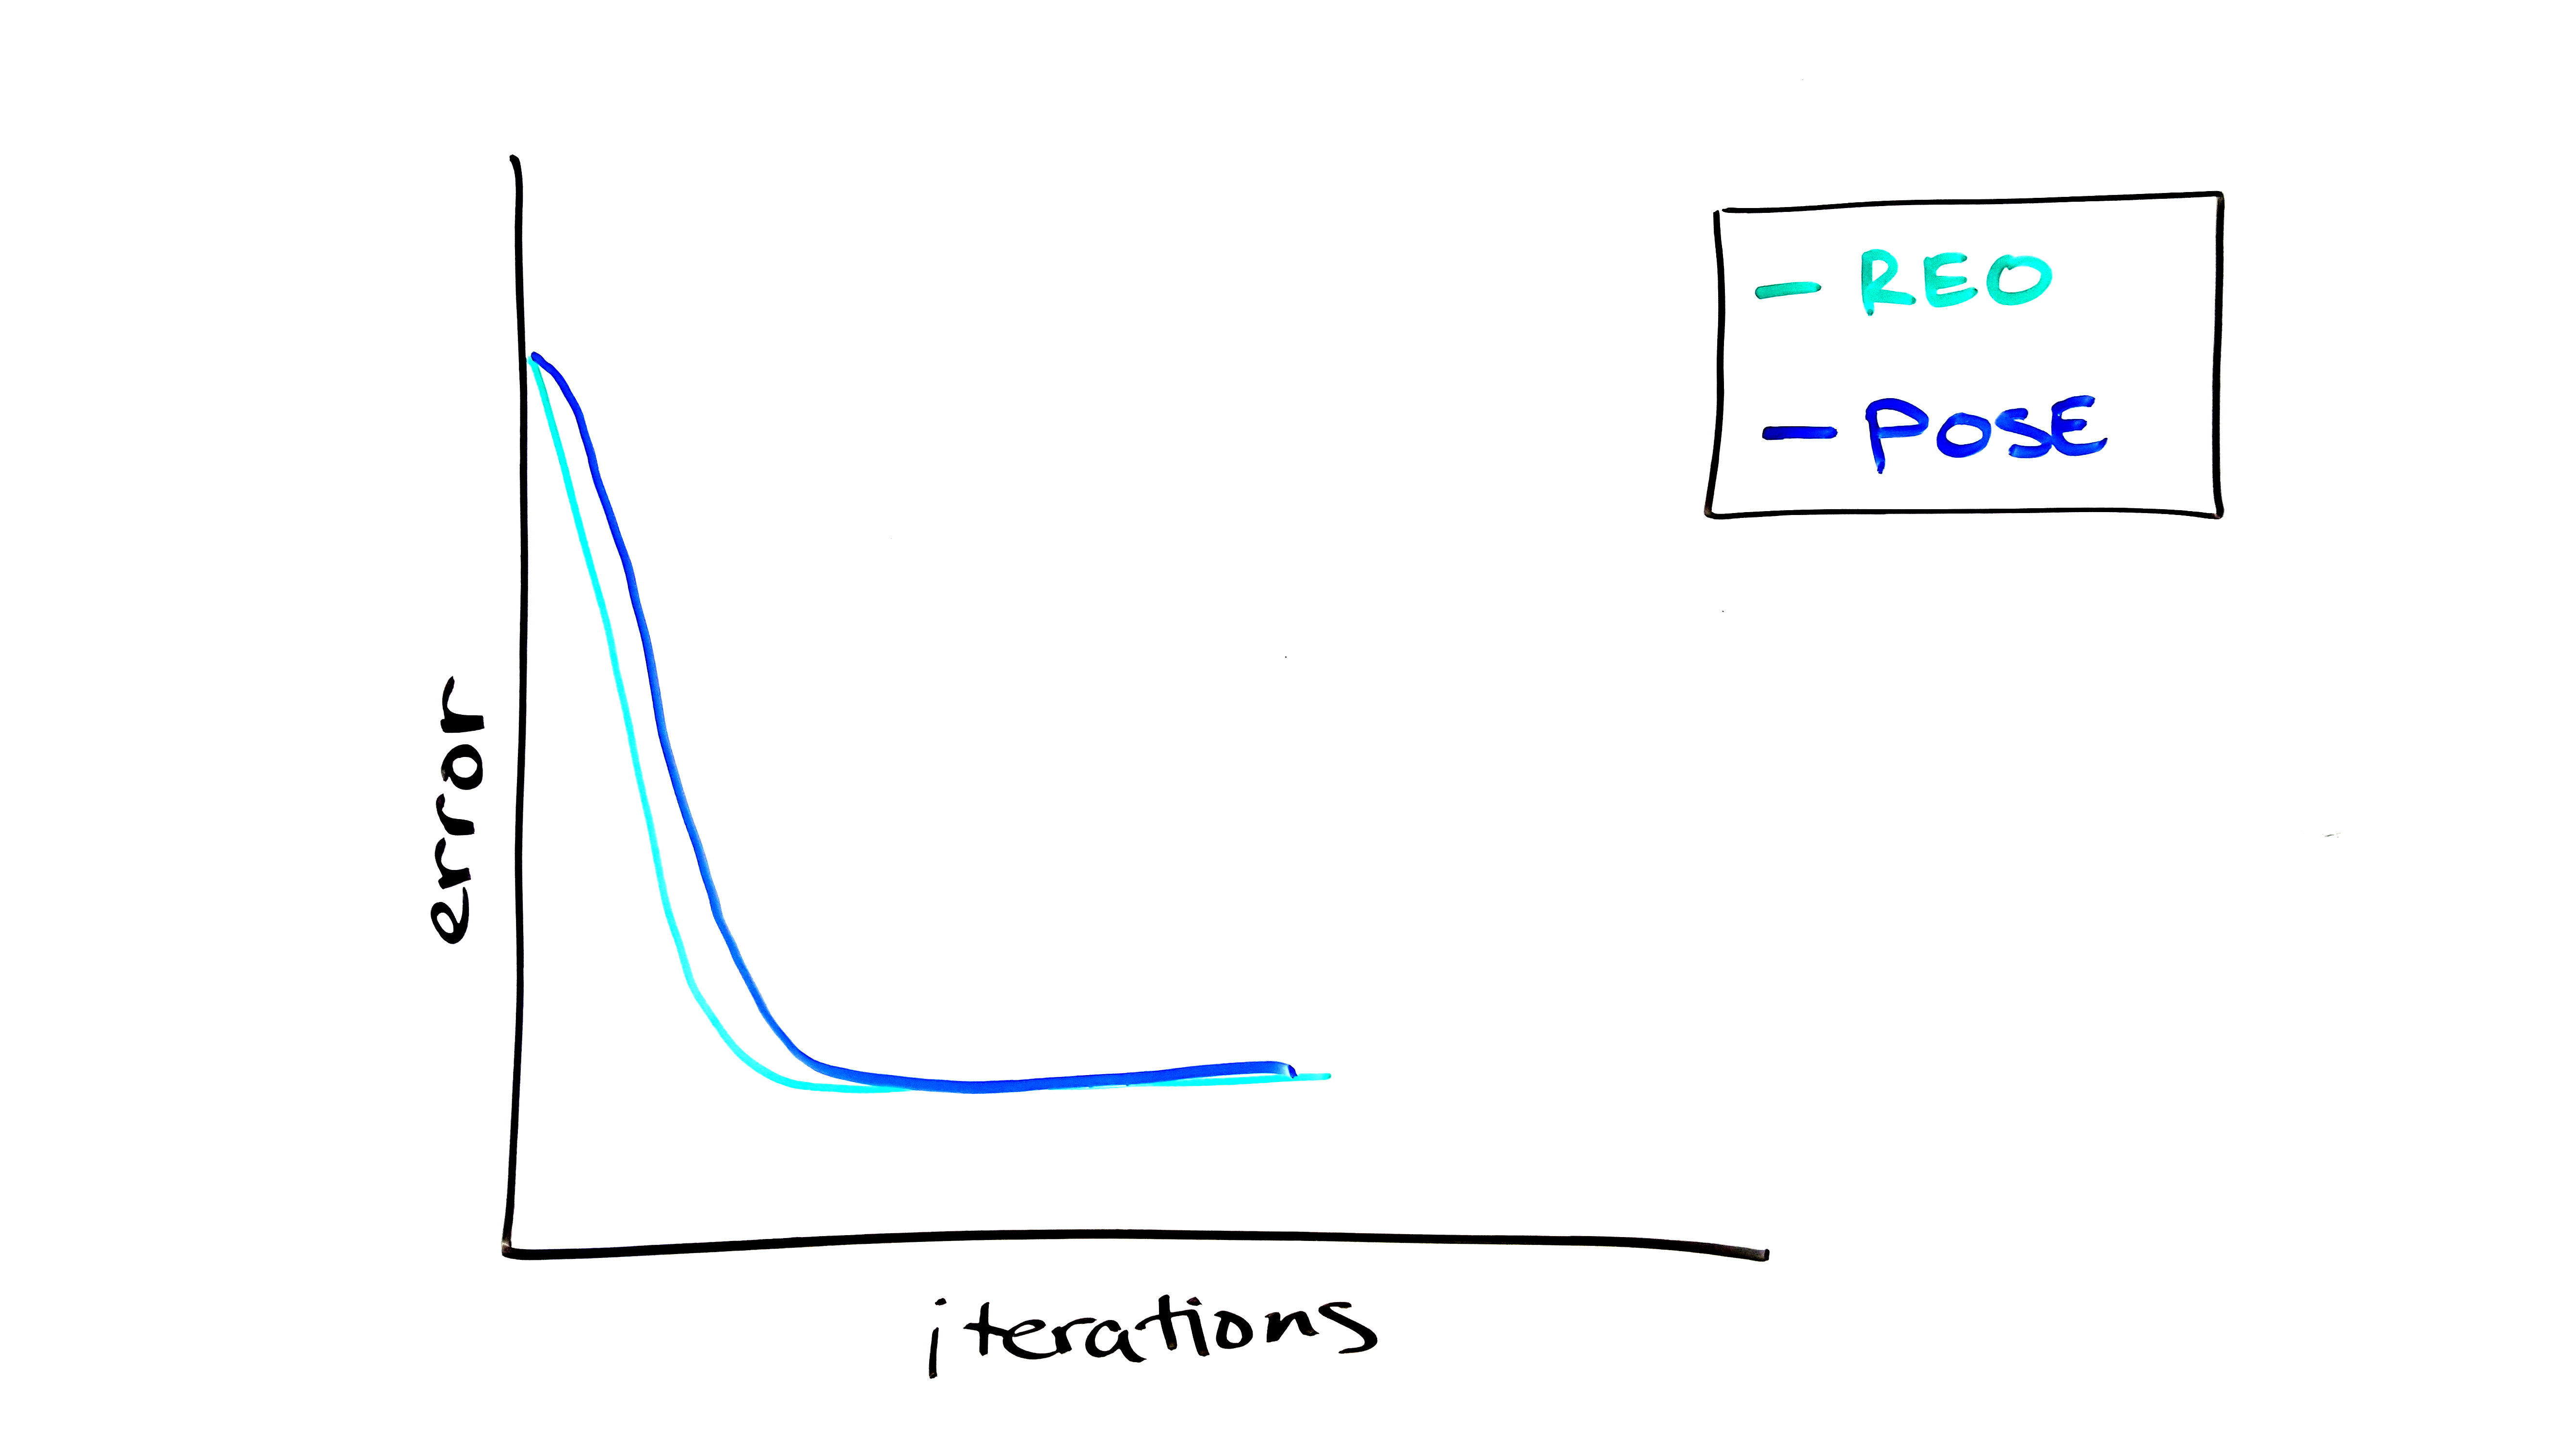
\includegraphics[width=0.7\textwidth]{figures/convergence_comparison_house.jpg}
  \caption{Convergence for the house trajectory}
  \label{fig:convergence_house}
\end{figure}

% show that they are equivalent
It can be plainly observed from comparing Eq~\ref{eqn:global_opt} and Eq~\ref{eqn:relative_opt} that relative edge optimization simply parametertizes the same cost function with relative edge constraints as opposed to global constraints, and therefore should result in an equivalent solution.  However, due to the different linearization between the two parameterizations, a simulation study was performed to show the equivalence of global pose and edge-based optimization. This was performed by optimization a house-shaped trajectory, shown in Figure~\ref{fig:house_trajectory} which was corrupted with random gaussian noise, had a random selction of edges were reversed and a loop closure placed between nodes at the bottom left corner of the trajectory. Every one of these optimizations produced identical results between global pose and edge-based optimization with a comparable number of iterations, shown in Figure~\ref{fig:convergence_house}.

% describe differences (pros/cons)
Differences between the performance of global pose graph and relative edge-based optimizations can be observed by stressing linearization errors in the various parameterizations.  For example, if the house trajectory is initialized with a 180$^\circ$ heading error, and provided global measurements, the global pose optimization often struggles to find the global minimum.  A similar experiment with 10,000 house trajectories was performed, except with the addition of a global measurement located at the peak of the house.  In this study, the pose graph optimization failed to converge to the correct optimum (As shown in Figure~\ref{fig:g2o_heading_divergence}) $20\%$ of the time, came to the same result but took more iterations as relative edge optimization $50\%$ of the time, and performed equivalently (same number of iterations, same result) the remaining $30\%$ of the time.

\begin{figure}[H]
  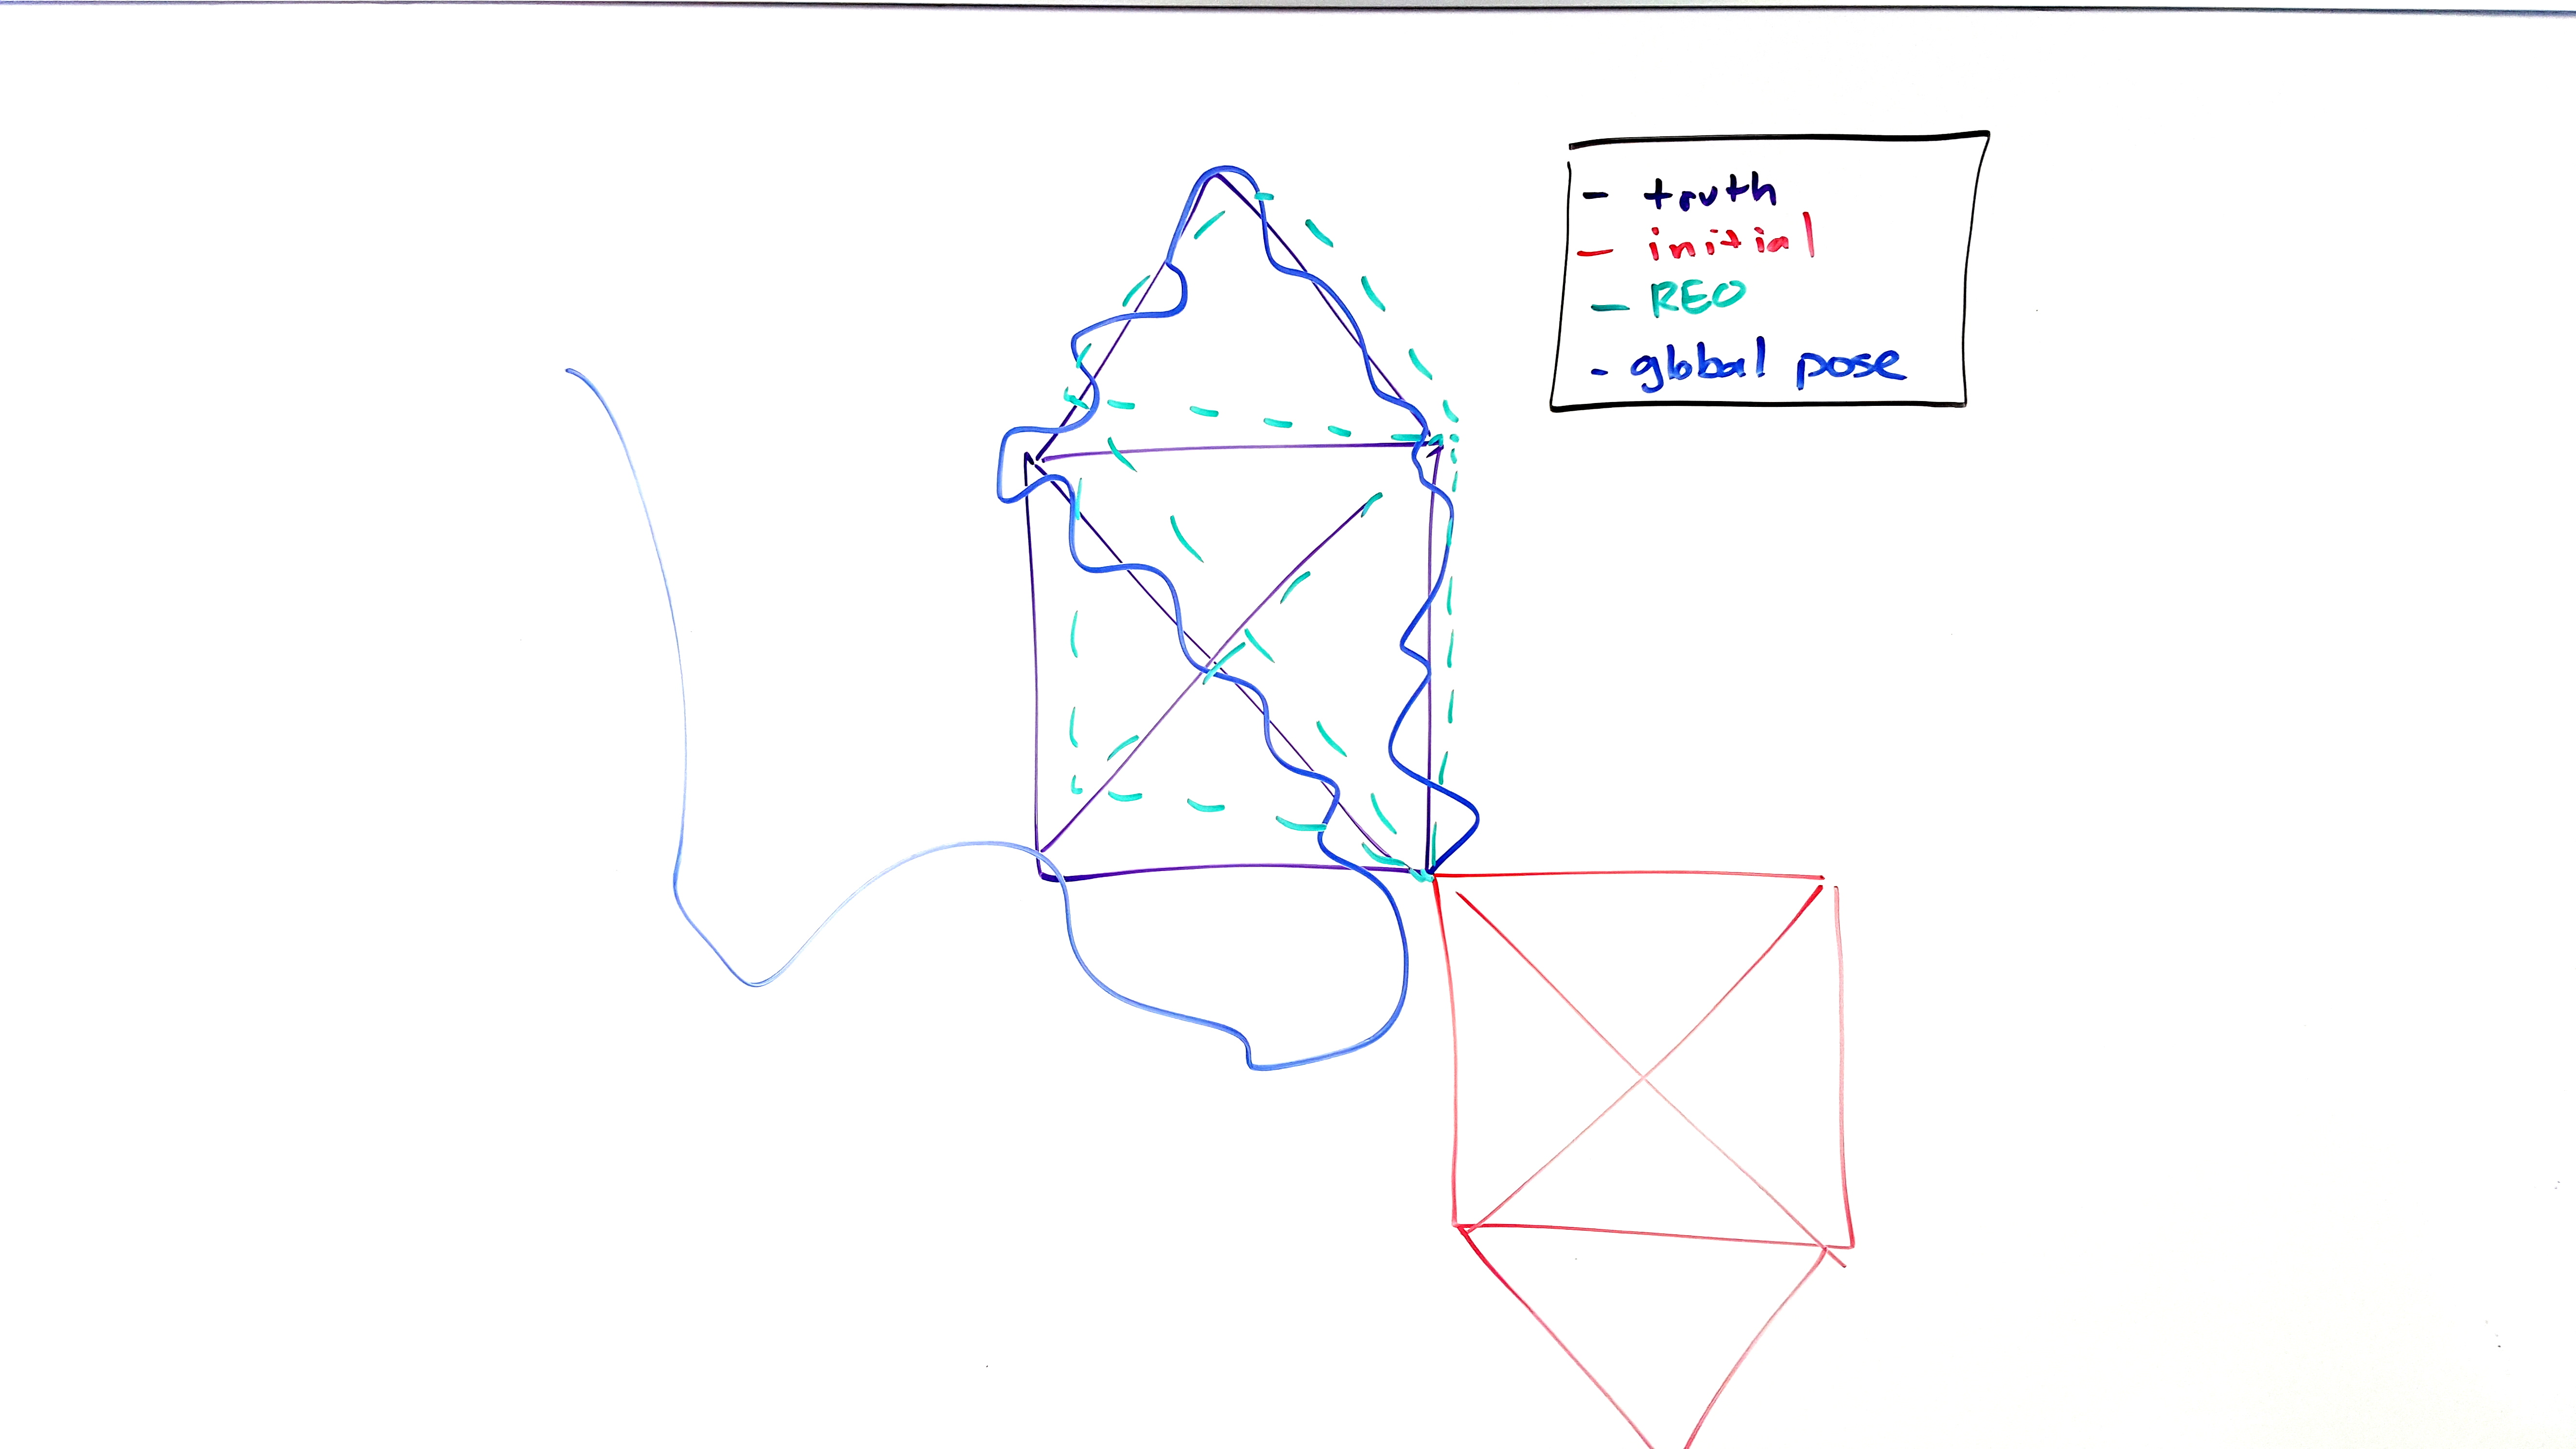
\includegraphics[width=0.7\textwidth]{figures/house_g2o_diverged.jpg}
  \caption{One sample from simulation study with a single global measurement added to peak of house trajectory,  initialized with a 180$^\circ$ heading error.  In this simulation, the global pose optimization failed to find the correct optimum.}
  \label{fig:g2o_heading_divergence}
\end{figure}

While relative edge optimization promises significant improvements in dealing with initialization errors when compared with global pose optimization, it is not as easily scaleable as global pose graph optimization.  In particular, the calculation of $\frac {\partial\Delta t_{a-z}}{\partial\Delta t_{ij}}$ causes significant correlations between edge estimates in a loop closure.  This ultimately leads to a loss of sparsity in the calculation of $\mathbf{H}_{az}^\top \Omega_{az} \mathbf{H}_{az}$ in Equation~\ref{eqn:3d_opt}.  The parameterization of global pose optimization however, does not run into this issue and can therefore exploit sparsity in solving for $\Delta \mathbf{x}$.  This becomes most important when considering a loop closure with a large number of edges where a dense matrix decomposition can be very costly. Secondly, in typical pose graph implementation, the number of edges can grow explosively if an agent repeatedly navigates the same area.  In this situation, the sum in the second term of the cost function in Equation~\ref{eqn:cost_function} can become extremely large and costly to calculate.


% how to use them together
To overcome these issue, we propose a two-fold solution.  To reduce the number of terms summed in the second term of Equation~\ref{eqn:cost_function}, we propose stochastically iterating over smaller loop closures in a well-connected pose graph and optimizing only a selection at a time.  To reduce the size of the optimization, we will exploit the relative nature of edge-based optimization to recursively break the full optimization into small, easy-to-manage problems.  This recursive process has the added benefit of producing completely parallelizeable independent computations which can be distributed to a GPU for fast evaluation.  While these solutions improve the scaleability of edge optimization, it still does not compete with the state-of-the-art global pose graph optimization libraries in terms of speed.  Due to the different parameterization, however, it can quickly bring a poorly initialized graph into a region where global pose graph optimization can quickly and reliably converge to a solution.  Therefore, we propose that edge optimization be performed for just a few iterations in situations where global pose graphs may struggle to find global minima to initialize the graph.  After much of the error has been removed by the more expensive, but less sensitive edge optimization, global pose graph optimization can very quickly find a global minima even in highly-connected and complicated graphs, where repeated edge optimization may become intractable.

% !TEX root=main.tex

\section{Hardware Implementation}
There are several important details which are critical to demonstrating an effective relative edge-based optimization in hardware.  We will now discuss these details as they pertain to implementation on a small multirotor robot.

% talk briefly about front-end implementation
% talk about how edges are created
% talk about simulation simplification, define what an edge means and why we are only doing SE2
% Talk about specific algorithms being used
\subsection{Front-end State Estimation}
Front-end state estimation must take place in real-time onboard a MAV. This state estimator must also provide mutually independent edge constraints to the back-end optimization routine.  In our implementation, we leverage the Relative Multiplicative Extended Kalman Filter (RMEKF)~\cite{Koch2017}, which has been demonstrated as an accurate filter-based front-end estimator which also provides mutually independent edge constraints to build a global pose graph.

As noted in~\cite{Wheeler2017a}, when operating a MAV over a flat ground plane, only the global position and heading states are unobservable to an agent equipped with relative sensors, an altimeter and an IMU.  Therefore, we only optimize over the unobservable states, which reduces the back-end optimization problem to transforms in $SE(2)$.  Therefore, we define edges as homogeneous transforms in $SE(2)$ as described in section~\ref{sec:relative_edge_optimization_in_se2}.

\subsection{Loop Closure Discovery and Calculation}
In addition to odometry constraints from the front-end estimation routine, we also require loop closure constraints when a vehicle observes landmarks it or another vehicle has viewed previously.  In our implementation, we utilize Fast, Appearance-Based Mapping (FAB-MAP) as our place-recognition algorithm and RGBD visual odometry techniques~\cite{Leishman2013} to calculate the full 6-Degree-Of-Freedom loop closure constraint between appearance-based matches.  These constraints have the same form as an odometry edge, and are also independent of other edges.  Therefore they can be considered homogeneously.

% !TEX root=main.tex

\section{Experimental Results}

Data was collected on a single multirotor agent, shown in~\ref{fig:leo_hardware}.  This agent was flown four times in a cluttered, GPS denied environment.  The agent was initalized in various locations with various initial headings but flew in trajectories which would provide sufficient overlap to calculate loop closures.  The data from each flight was saved and post-processed by the same onboard computer as if all flights were being performed simultaneously by different agents connected to the same ROS network.  The optimized route of each agent can be seen in figure~\ref{fig:hardware_results}.  Each flight took about 2 minutes, and traversed on average about 100m.

\begin{figure}[H]
  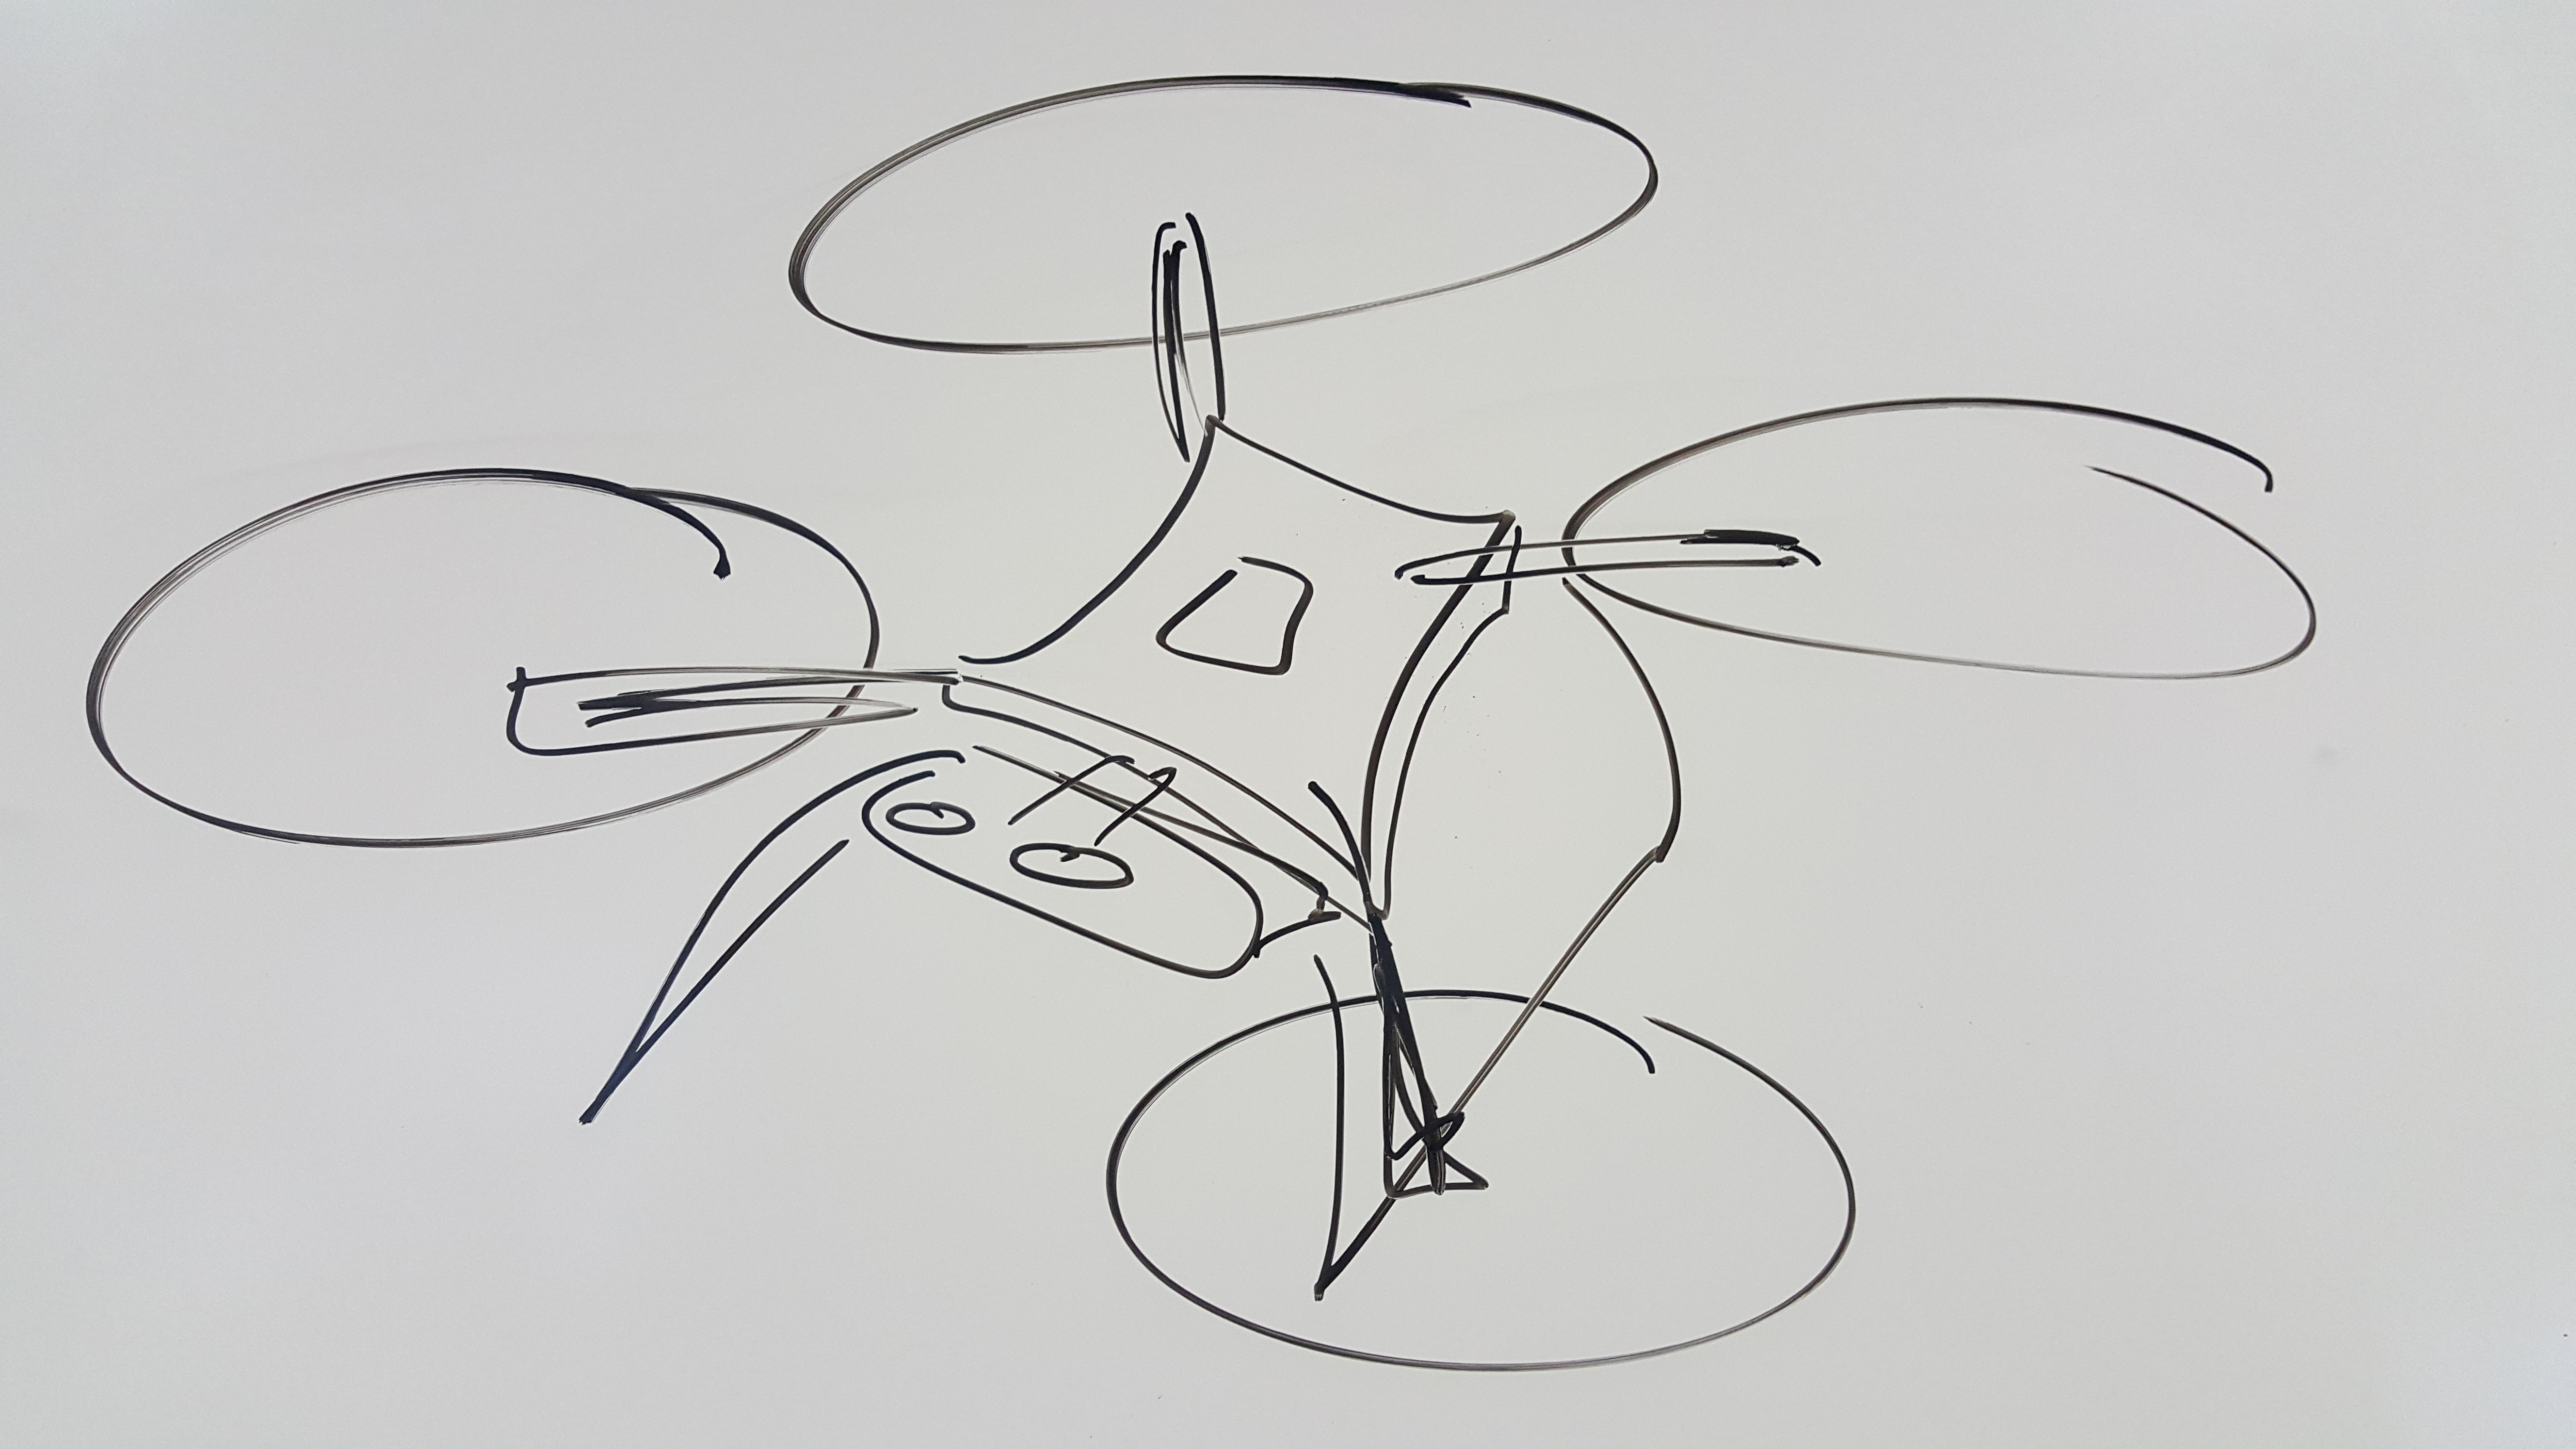
\includegraphics[width=0.7\textwidth]{figures/leo.jpg}
  \caption{Multirotor used in testing.  Processing was performed by an onboard computer with i7-4660U dual core processor and 16GB RAM.  An ASUS XTION RGBD camera was used to provide visual odometry which was fed to an RMEKF which fused MEMS IMU sensor readings and sonar altimeter information collected by a flip32 flight control board running ROSflight.}
  \label{fig:leo_hardware}
\end{figure}


\begin{figure}[H]
  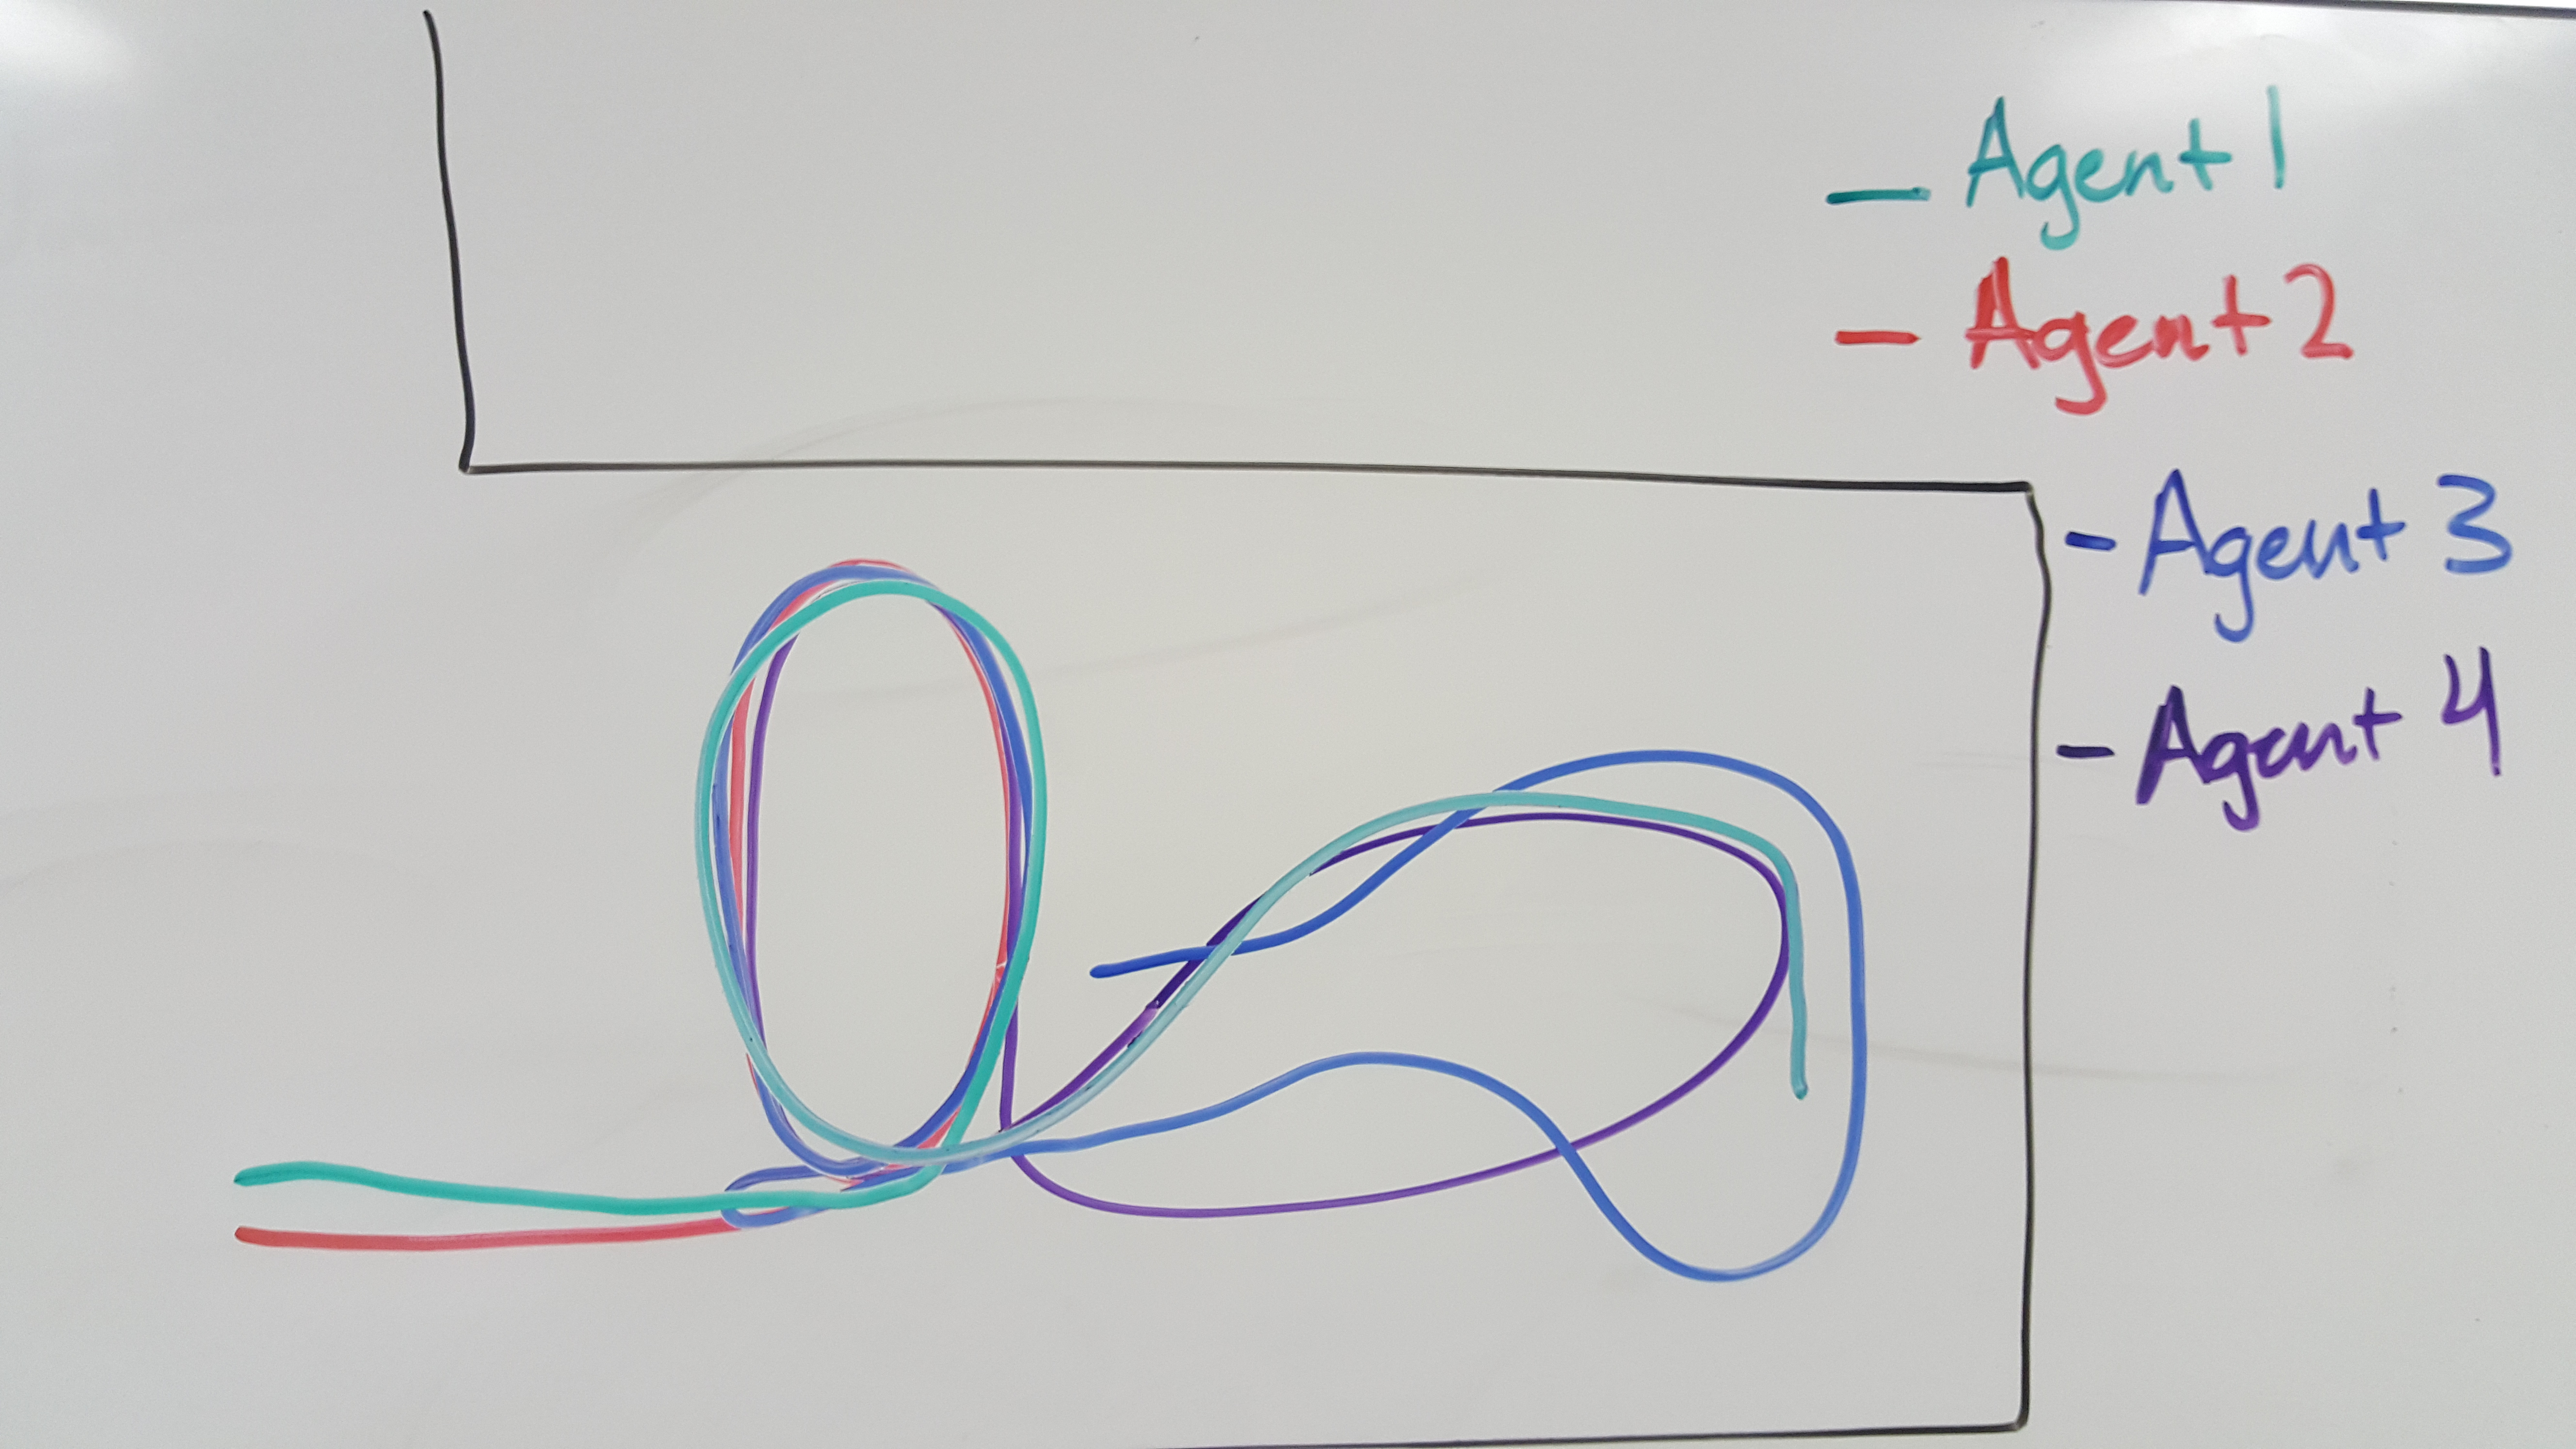
\includegraphics[width=0.7\textwidth]{figures/hardware_results.jpg}
  \caption{Multirotor used in testing.  Processing was performed by an onboard computer with i7-4660U dual core processor and 16GB RAM.  An ASUS XTION RGBD camera was used to provide visual odometry which was fed to an RMEKF which fused MEMS IMU sensor readings and sonar altimeter information collected by a flip32 flight control board running ROSflight.}
  \label{fig:hardware_results}
\end{figure}

This experiment was repeated two times.  In the first experiment, a python implementation of REO was used to as the sole optimization routine.  Optimization was performed once per second on all available information from the perspective of the first agent.  Optimization was performed as a batch, initialized with raw odometry and loop closure measurements.  The optimization always converged in less than 30 iterations for the entirety of the experiment.  On average, optimizations took about 0.1s, but the time to optimization grew as the combined graph got more complicated.

The second experiment used REO only to initialize new agents, aligning them with the primary graph by performing 3 iterations of optimization on the smallest set of edges which forms a loop that includes two agents.   After this initial alignment phase, GPO was used to quickly converge to an estimate.  This resulted in a fixed-cost add to the optimization routine, as the cost of performing REO did not change with increasingly complicated graphs.  GPO also scales non-linearly with increasing graph complexity, but not as strongly as REO.  Therefore it is much more reasonable to use in large networks of agents.

\begin{figure}[H]
  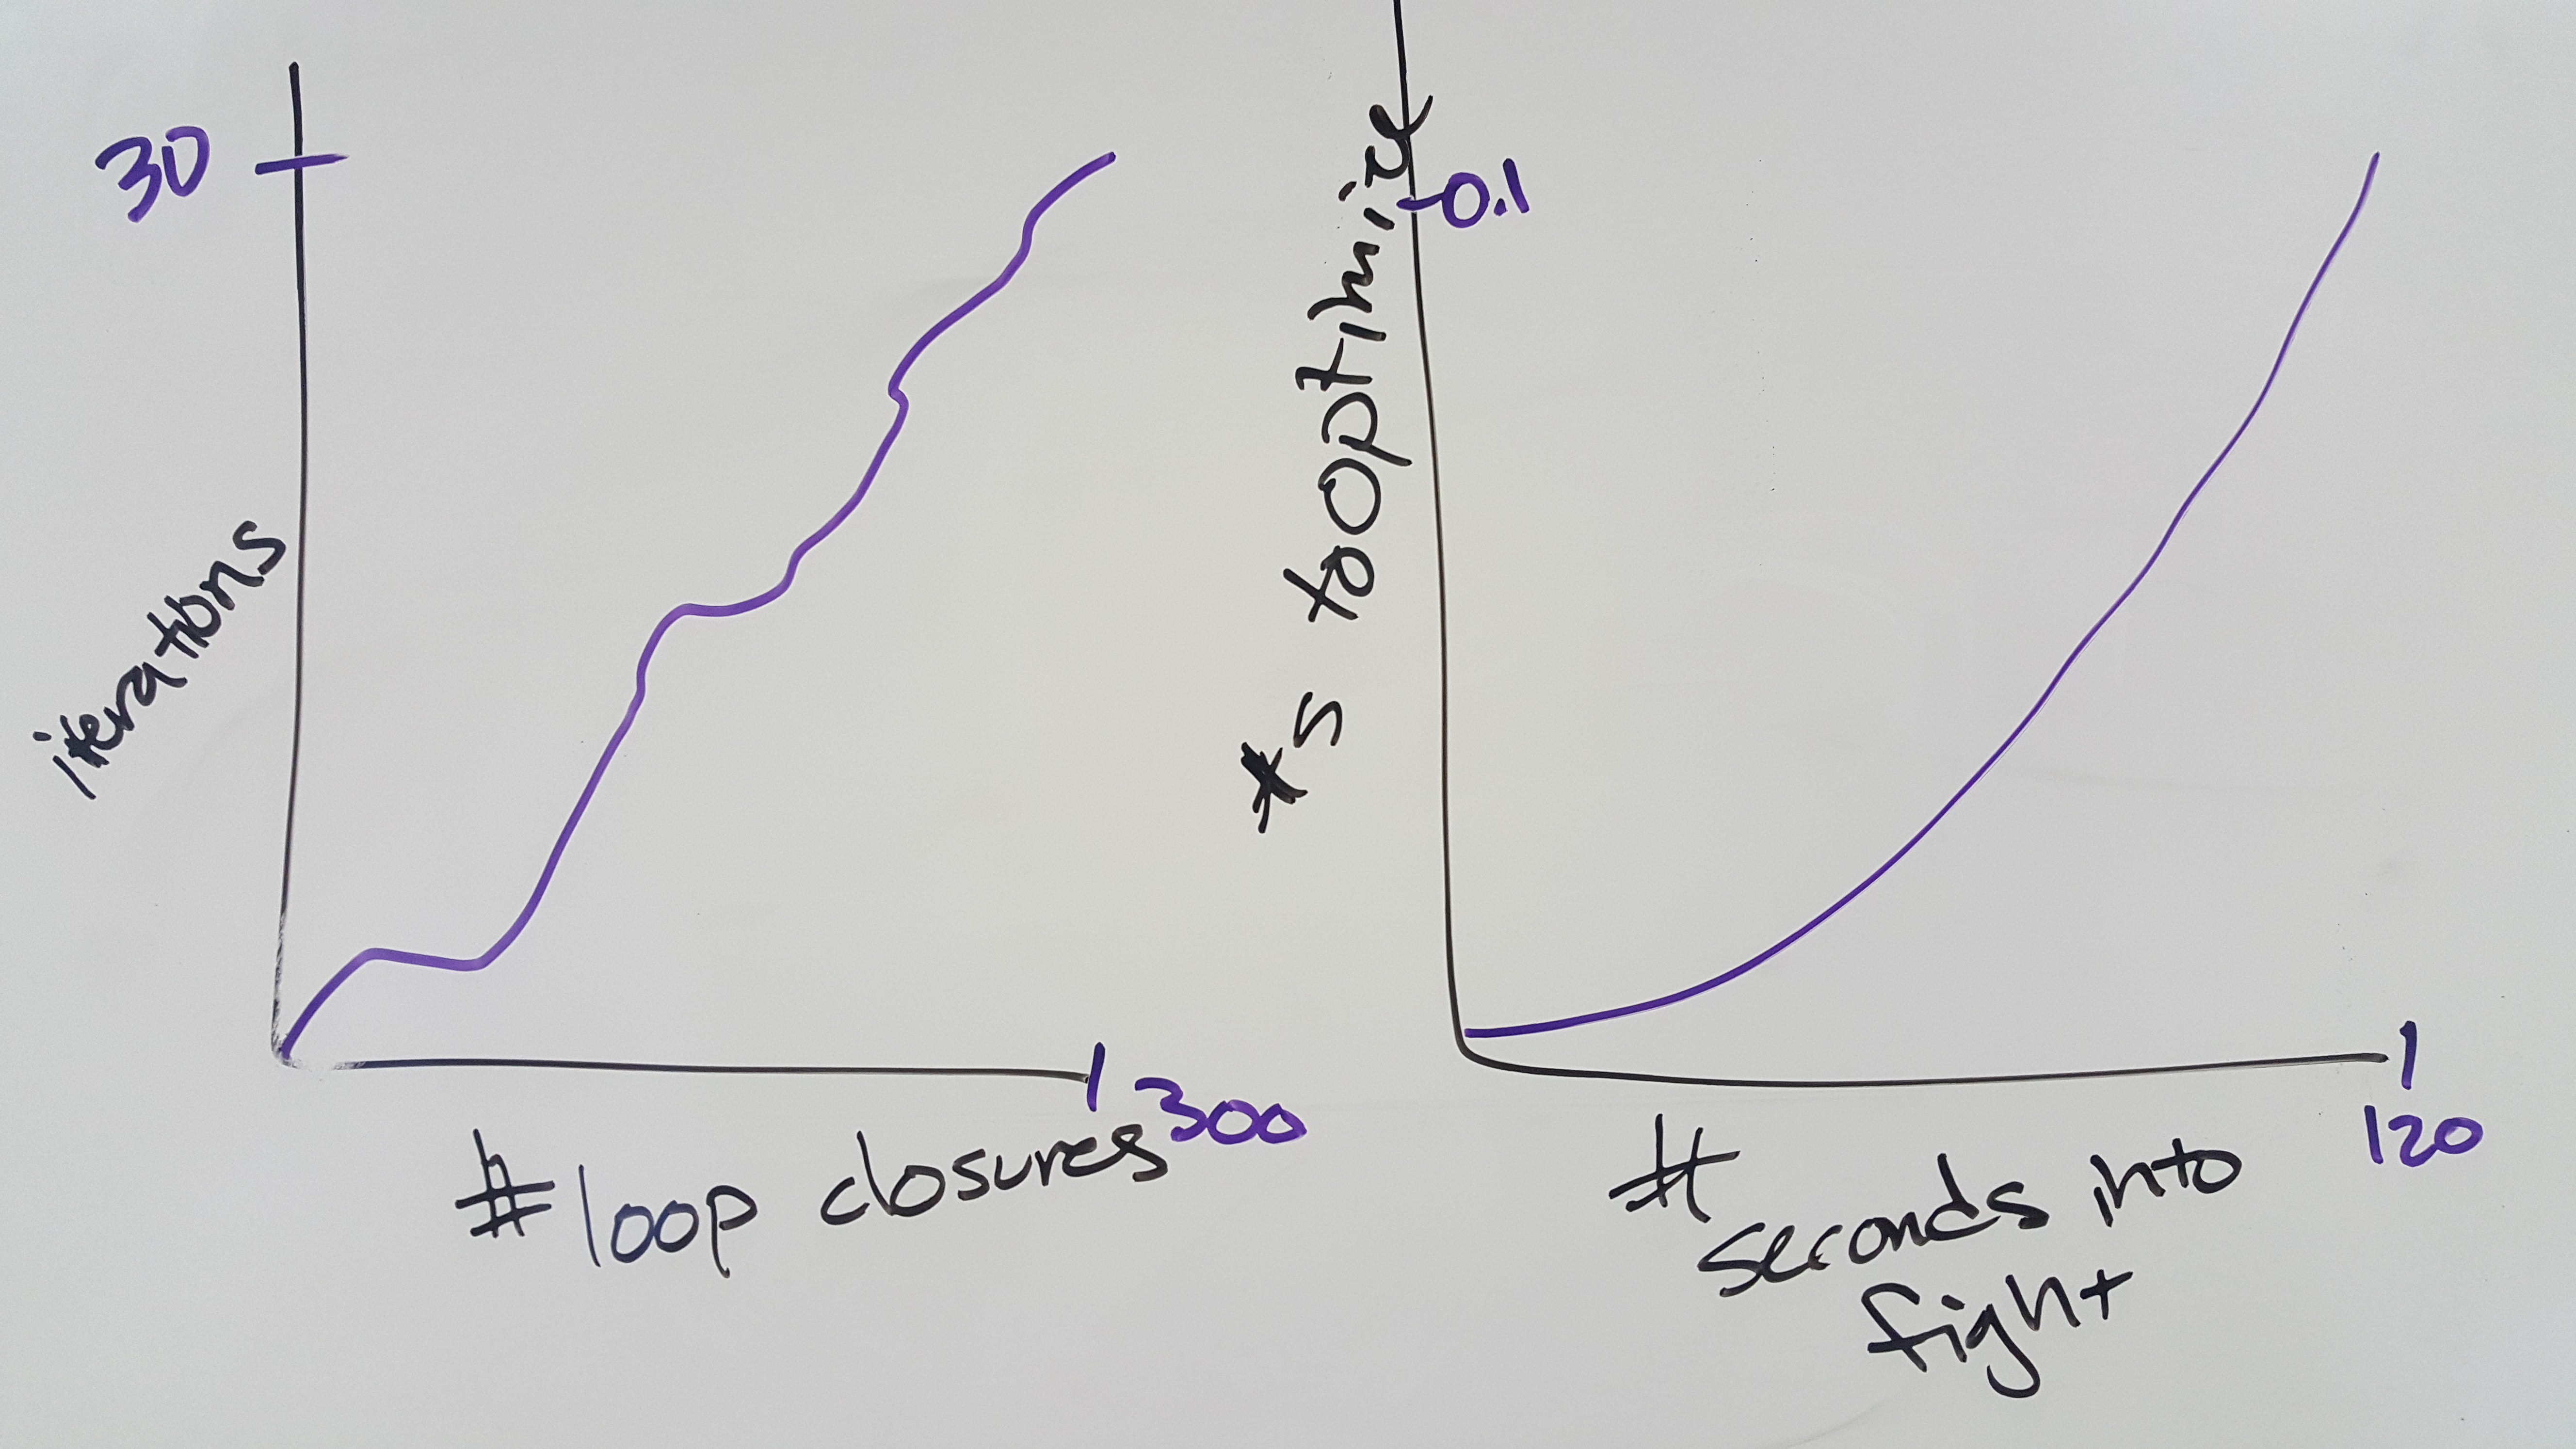
\includegraphics[width=0.7\textwidth]{figures/REO_only_timing_results.jpg}
  \caption{Average number of iterations of REO vs the number of loop closures discovered in the system and average number of seconds to optimize vs the number of seconds into the flight.  While REO was able to perform in real time for this experiment, large scale experiments could pose a challenge for a REO-only backend}
  \label{fig:REO_only_hardware_results}
\end{figure}

% !TEX root=main.tex

\section{Conclusions}

% Pose graphs and relative navigation setups are a scaleable way to make a multi-agent MAV system
% Edge optimization is helpful in initializing pose graph optimizations
% Edge optimization can help avoid graph divergence
% Using stochastic gradient descent in edge optimization can help reduce burden with a large number of edges
% Future work - Better understanding of how to detect incorrect loop closures with edge optimization


\end{spacing}

% \section*{Acknowledgment}
%
%
% The authors would like to thank...

\bibliographystyle{ieeetr}
\bibliography{library}
\end{document}
